%
% Portuguese-BR vertion
% 
\documentclass{article}

\usepackage{ipprocess}
% Use longtable if you want big tables to split over multiple pages.
% \usepackage{longtable}
\usepackage[utf8]{inputenc} 
\usepackage[brazil]{babel} % Uncomment for portuguese
\usepackage{tikz}
\usepackage{tikz-uml}

\sloppy

\graphicspath{{./pictures/}} % Pictures dir
\makeindex
\begin{document}

\DocumentTitle{Documento de Casos de Uso}
\Project{Unidade de Operações Aritméticas}
\Organization{Universidade Estadual de Feira de Santana}
\Version{Build 2.0a}

\capa
\newpage

%%%%%%%%%%%%%%%%%%%%%%%%%%%%%%%%%%%%%%%%%%%%%%%%%%
%% Revision History
%%%%%%%%%%%%%%%%%%%%%%%%%%%%%%%%%%%%%%%%%%%%%%%%%%
\section*{\center Histórico de Revisões}
  \vspace*{1cm}
  \begin{table}[ht]
    \centering
    \begin{tabular}[pos]{|m{2cm} | m{7.2cm} | m{3.8cm}|} 
      \hline
      \cellcolor[gray]{0.9}
      \textbf{Date} & \cellcolor[gray]{0.9}\textbf{Descrição} & \cellcolor[gray]{0.9}\textbf{Autor(s)}\\ \hline
      \small 18/08/2014 & \small Document conception & \small joaocarlos \\ \hline      
    \end{tabular}
  \end{table}

\newpage

% TOC instantiation
\tableofcontents
\newpage

%%%%%%%%%%%%%%%%%%%%%%%%%%%%%%%%%%%%%%%%%%%%%%%%%%
%% Document main content
%%%%%%%%%%%%%%%%%%%%%%%%%%%%%%%%%%%%%%%%%%%%%%%%%%
\section{Introdução}

  \subsection{Objetivo}
  O objetivo desse documento é especificar os casos de uso do projeto \ipPROCESSProject. O documento contempla as seguintes informações: descrição dos Atores envolvidos no processo; definição dos fluxos de eventos principal e secundário; lista de requisitos especiais, funcionais e não funcionais; estabelecimento de pré-condições e pós-condições.

  \subsection{Visão Geral do Documento}
  \begin{itemize}
    \item Sessão 2: lista todos os possíveis atores do sistema.
    \item Sessão 3: relata a lista dos casos de uso do projeto.
    % \item Referências: provê uma lista completa de todos os artefatos referenciados nesse documento.
  \end{itemize}
  
  \subsection{Representação Simbólica}
  A Figura \ref{fig:uc_exemple} ilustra a simbologia utilizada para representar operações que devem ser realizadas pelo sistema. A Figura \ref{fig:actors} ilustra as duas simbologias utilizadas para representar os Atores do sistema. Um ator, dentro do escopo desta descrição, pode ser identificado como um módulo \textit{top level}, ou como um elemento de entrada e saída (botões, sensores, displays, etc).
  
  % \FloatBarrier
  % \begin{figure}[H]
  %   \centering
  %   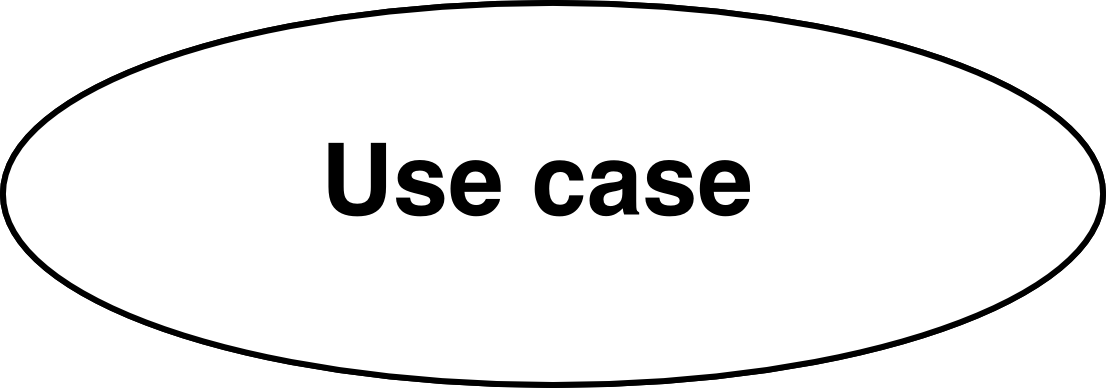
\includegraphics[width=0.25\textwidth]{uc_exemple.png}
  %   \caption{Exemplo de Caso de Uso.}
  %   \label{fig:uc_exemple}
  % \end{figure}
    \begin{figure}[H]
      \centering
      \begin{tikzpicture} 
        \umlusecase[name=usecase]{Caso de Uso}
      \end{tikzpicture}  
      \caption{Exemplo de Caso de Uso.}
      \label{fig:uc_exemple}
    \end{figure}
  
  A simbologia usual para representação de um Ator é apresentada na Figura \ref{fig:actor_exemple}, no entanto, para representar módulos incorporados que outrora deveriam utilizar a mesma simbologia, utiliza-se a representação ilustrada nas Figuras \ref{fig:ipcore_exemple} e \ref{fig:ipcore_single_exemple}, definida por convenção. Este elemento, em geral, está associado aos módulos do sistema, ou IP-cores que de terceiros incorporados ao mesmo. Esta simbologia ainda foi divida, tendo em vista representar instâncias únicas (Figura \ref{fig:ipcore_single_exemple}), ou múltiplas (Figura \ref{fig:ipcore_exemple}) de um determinado componente. 
  
  \FloatBarrier
  \begin{figure}[H]
    \centering
    \begin{subfigure}[b]{0.3\textwidth}
      \centering
      \begin{tikzpicture} 
        \umlactor{Ator}
      \end{tikzpicture}
      \caption{Ator do Sistema.}
      \label{fig:actor_exemple}
    \end{subfigure} 
    \begin{subfigure}[b]{0.3\textwidth}
      \centering
      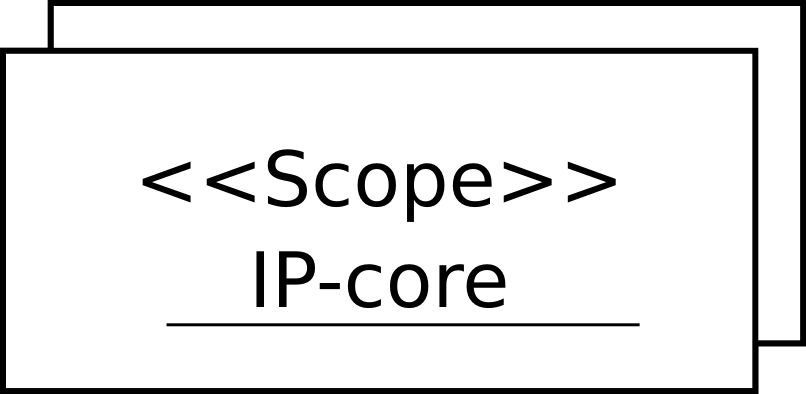
\includegraphics[width=0.6\textwidth]{ipcore_exemple.png}
      \caption{Instância múltipla de um IP.}
      \label{fig:ipcore_exemple}
    \end{subfigure}
    \begin{subfigure}[b]{0.3\textwidth}
      \centering
      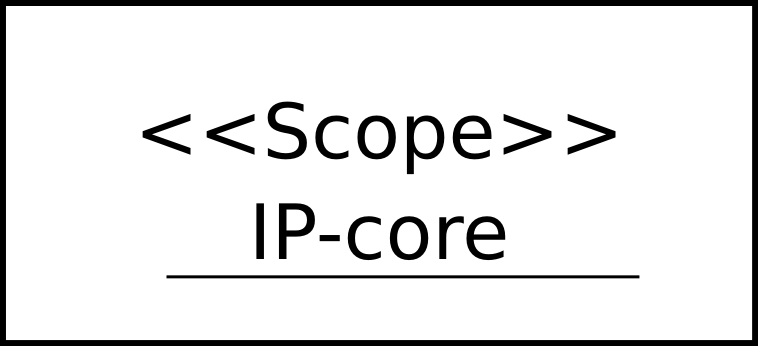
\includegraphics[width=0.6\textwidth]{ipcore_single_exemple.png}
      \caption{Instância de um IP.}
      \label{fig:ipcore_single_exemple}
    \end{subfigure}
    \caption{Simbologia utilizada na implementação dos Casos de Uso.}
    \label{fig:actors}
  \end{figure}
  
  O projetista responsável por interpretar os diagramas não deve confundir-se no momento de interpretar as simbologias de atores. A representação alternativa, não implica que o módulo será instanciado no subsistema em questão, mas sim que os recursos providos por este \textit{core} são necessários para garantir o seu funcionamento.
  
  \subsection{Definições, Acrônimos e Abreviações}
  \FloatBarrier
    \begin{table}[H] 
      \begin{center}
        \begin{tabular}[pos]{|m{2cm} | m{8cm}|} 
          \hline 
          \cellcolor[gray]{0.9}\textbf{Termo} & \cellcolor[gray]{0.9}\textbf{Descrição} \\ \hline
          UC & Caso de Uso  \\ \hline
          SF & Fluxo Secundário \\ \hline
          FR & Requisito Funcional \\ \hline
          LED & Light Emitter Diode \\ \hline
          IF & Interface \\ \hline
        \end{tabular}
      \end{center}
    \label{tab:definicoes}
    \end{table}

  \section{Atores do Sistema}

  \begin{figure}[H]
    \centering
    \begin{tikzpicture} 
      \umlactor{Controle IF} 
      \umlactor[x=2]{Controle}
      \umlactor[x=4]{LED de dados} 
      \umlactor[x=6.5]{LED de overflow}  
    \end{tikzpicture} 
  \end{figure}

  \begin{description}
    \actor{Controle IF}{Entidade responsável por controlar os pacotes de entrada de dados.}    
    \actor{Controle}{Unidade que controla a execução das operações.}
    \actor{LED de overflow}{Interface de saída que aciona o LED de overflow.}
    \actor{LEDs de dados:}{Interface de saída que aciona os sinais de dados.}
  \end{description}

  \section{Casos de Usos}

  \usecase{Unidade de Processamento}
  A \textbf{Unidade de Processamento} é responśavel por realizar as operações aritméticas e lógicas, de acordo com o código de entrada.
  
  \actors
    \begin{description}
     \actor{Controle}{Unidade que controla a execução das operações.}
     \actor{LED de overflow}{Interface de saída que aciona o LED de overflow.}
     \actor{LEDs de dados:}{Interface de saída que aciona os sinais de dados.}
    \end{description}
  
  \preconditions 
    \begin{itemize}
     \item Atender aos requisitos funcionais [FR7-12];
     \item Codificação das operações deve ser definida;
     \item Identificação das unidades sequenciais e combinacionais;
    \end{itemize}

  \postconditions
    \begin{itemize}
     \item O módulo deve ser capaz de detectar overflow aritmético;
     \item O resultado deve estar presente nas saídas correspondentes aos pinos de dados usando uma codificação binária;
    \end{itemize}
  
  % \ucdiagram{./pictures/uc_exemple.png}
  \subsubsection*{Diagrama de Caso de Uso}
    \flushleft
  \begin{tikzpicture} 
    \begin{umlsystem}[x=0, fill=red!10]{Unidade de Processamento} 
      \umlusecase[x=-3,y=-5,name=decod]{Decodificar} 
      \umlusecase[name=soma]{Somar} 
      \umlusecase[y=-2, name=subtrai]{Subtrair} 
      \umlusecase[y=-4, name=mult]{Multiplicar} 
      \umlusecase[y=-6, name=div]{Dividir} 
      \umlusecase[y=-8, name=and]{AND}
      \umlusecase[y=-10, name=or]{OR}
      \umlusecase[x=4,y=-6, width=1.5cm, name=processa]{Processar resultado}   
      \umlusecase[x=4,y=-3, fill=green!20,width=1cm, name=flags]{Definir flags} 

      \umlactor[x=-6,y=-5]{Controle} 
      \umlactor[x=7.5,y=-6]{LED de dados} 
      \umlactor[x=7.5, y=-3]{LED de overflow}   

      \umlassoc{Controle}{decod}
      \umlassoc{decod}{soma}
      \umlassoc{decod}{subtrai}
      \umlassoc{decod}{mult}
      \umlassoc{decod}{div}
      \umlassoc{decod}{and}
      \umlassoc{decod}{or}
      \umlassoc{processa}{LED de dados}
      \umlassoc{soma}{flags}
      \umlassoc{subtrai}{flags}
      \umlassoc{mult}{flags}
      \umlassoc{div}{flags}
      \umlassoc{flags}{LED de overflow}
      \umlinclude{soma}{processa}
      \umlinclude{subtrai}{processa}
      \umlinclude{mult}{processa}
      \umlinclude{div}{processa}
      \umlinclude{and}{processa}
      \umlinclude{or}{processa}
    \end{umlsystem} 
  \end{tikzpicture} 
 
  
  % descricao do fluxo principal de eventos
  \begin{mainflow}
    \item Decodificar o indicador operação;
    \item Realizar operação aritmética ou lógica;
    \item Armazenar o resultado em um registrador;
  \end{mainflow}
  
  % descricao do fluxo secundário (quando existir)
  \begin{secondaryflow} 
    \sfitem{Valor do resultado excede o suportado}
    \begin{enumerate}
      \item Habilitar sinal de overflow;
    \end{enumerate}
  \end{secondaryflow}  

  \usecase{Interface de Comunidação}
  A \textbf{Interface de Comunicação} é responsável por estabelecer um mecanismo de interfaceamento entre as unidades de processamento e comunicação.
  
  \actors
    \begin{description}
     \actor{Controle IF}{Entidade responsável por controlar os pacotes de entrada de dados.}
     \actor{Controle}{Unidade que controla a execução das operações.}
    \end{description}
  
  \preconditions 
    \begin{itemize}
     \item Atender aos requisitos [FR2-4];
    \end{itemize}

  \postconditions
    \begin{itemize}
     \item O módulo deve transmitir as informações recebidas de forma paralela;
    \end{itemize}
  
  \newpage
  % \ucdiagram{./pictures/uc_exemple.png}
  \subsubsection*{Diagrama de Caso de Uso}
        \begin{tikzpicture} 
        \umlclass[type=control]{Interface\_Control}
        { % atributos
          + clock : input bit \\
          + reset : input bit \\
          + rx\_data\_ready : input bit \\
          + rx\_data : input bit[8] \\
          + data\_a : output bit[8] \\
          + data\_b : output bit[8] \\
          + operation : output bit[TBD] \\
          - state : reg bit[TBD] \\
          - data\_a\_reg : reg bit[8] \\
          - data\_b\_reg : reg bit[8] \\
          - operation\_reg : output bit[8]
        }{ % procedures
          - \underline{<<sequ>> control\_logic()} \\
          - <<sequ>> register\_assignment()
        }
      \end{tikzpicture}
  % descricao do fluxo principal de eventos
  \begin{mainflow}
    \item Realizar leitura do código da operação;
    \item Realizar leitura do primeiro operando;
    \item Realizar leitura do segundo operando;
    \item Disponibilizar dados na saída para o \textbf{Controle};
  \end{mainflow}
  
% Optional bibliography section
% To use bibliograpy, first provide the ipprocess.bib file on the root folder.
% \bibliographystyle{ieeetr}
% \bibliography{ipprocess}

\end{document}
